%%%%%%%%%%%%%%%%%%%%%%%%%%%%%%%%%%%%%%%%%
% Beamer Presentation
% LaTeX Template
% Version 1.0 (10/11/12)
%
% This template has been downloaded from:
% http://www.LaTeXTemplates.com
%
% License:
% CC BY-NC-SA 3.0 (http://creativecommons.org/licenses/by-nc-sa/3.0/)
%
%%%%%%%%%%%%%%%%%%%%%%%%%%%%%%%%%%%%%%%%%

%----------------------------------------------------------------------------------------
%	PACKAGES AND THEMES
%----------------------------------------------------------------------------------------

\documentclass[aspectratio=169]{beamer}
%\documentclass{beamer}

\mode<presentation> {

% The Beamer class comes with a number of default slide themes
% which change the colors and layouts of slides. Below this is a list
% of all the themes, uncomment each in turn to see what they look like.

%\usetheme{default}
%\usetheme{AnnArbor}
%\usetheme{Antibes}
%\usetheme{Bergen}
%\usetheme{Berkeley}
%\usetheme{Berlin}
%\usetheme{Boadilla}
%\usetheme{CambridgeUS}
%\usetheme{Copenhagen}
%\usetheme{Darmstadt}
%\usetheme{Dresden}
%\usetheme{Frankfurt}
%\usetheme{Goettingen}
%\usetheme{Hannover}
%\usetheme{Ilmenau}
%\usetheme{JuanLesPins}
%\usetheme{Luebeck}
\usetheme{Madrid}
%\usetheme{Malmoe}
%\usetheme{Marburg}
%\usetheme{Montpellier}
%\usetheme{PaloAlto}
%\usetheme{Pittsburgh}
%\usetheme{Rochester}
%\usetheme{Singapore}
%\usetheme{Szeged}
%\usetheme{Warsaw}

% As well as themes, the Beamer class has a number of color themes
% for any slide theme. Uncomment each of these in turn to see how it
% changes the colors of your current slide theme.

%\usecolortheme{albatross}
%\usecolortheme{beaver}
%\usecolortheme{beetle}
%\usecolortheme{crane}
%\usecolortheme{dolphin}
%\usecolortheme{dove}
%\usecolortheme{fly}
%\usecolortheme{lily}
%\usecolortheme{orchid}
%\usecolortheme{rose}
%\usecolortheme{seagull}
%\usecolortheme{seahorse}
%\usecolortheme{whale}
%\usecolortheme{wolverine}

%\setbeamertemplate{footline} % To remove the footer line in all slides uncomment this line
%\setbeamertemplate{footline}[page number] % To replace the footer line in all slides with a simple slide count uncomment this line

%\setbeamertemplate{navigation symbols}{} % To remove the navigation symbols from the bottom of all slides uncomment this line
}

\usepackage{graphicx} % Allows including images
\usepackage{booktabs} % Allows the use of \toprule, \midrule and \bottomrule in tables
%\RequirePackage{beamerthemeoracle}

%----------------------------------------------------------------------------------------
%	TITLE PAGE
%----------------------------------------------------------------------------------------

\title[The Philosophy in PCI Passthrough]{The Philosophy in PCI Passthrough} % The short title appears at the bottom of every slide, the full title is only on the title page

\author{Dongli Zhang} % Your name
%\institute[Oracle] % Your institution as it will appear on the bottom of every slide, may be shorthand to save space
%{
%Oracle Asia Research and Development Centers (Beijing) \\ % Your institution for the title page
%\medskip
%\textit{dongli.zhang@oracle.com} % Your email address
%}
\date{\today} % Date, can be changed to a custom date

\begin{document}

%------------------------------------------------

\section{Title}
\begin{frame}
\titlepage % Print the title page as the first slide
\end{frame}

%------------------------------------------------

\section{What is PCI passthrough?}
\begin{frame}
\frametitle{What is PCI passthrough?}
\begin{itemize}
\item To assign full and direct access of PCI device to VM
\visible<2->{\item How to assign bugs related to NVMe PCI passthrough?}
\begin{itemize}
\visible<3->{\item The NVMe developers may blame virtualization developers}
\visible<4->{\item The virtualization developers may blame hardware/firmware}
\end{itemize}
\end{itemize}
\begin{figure}
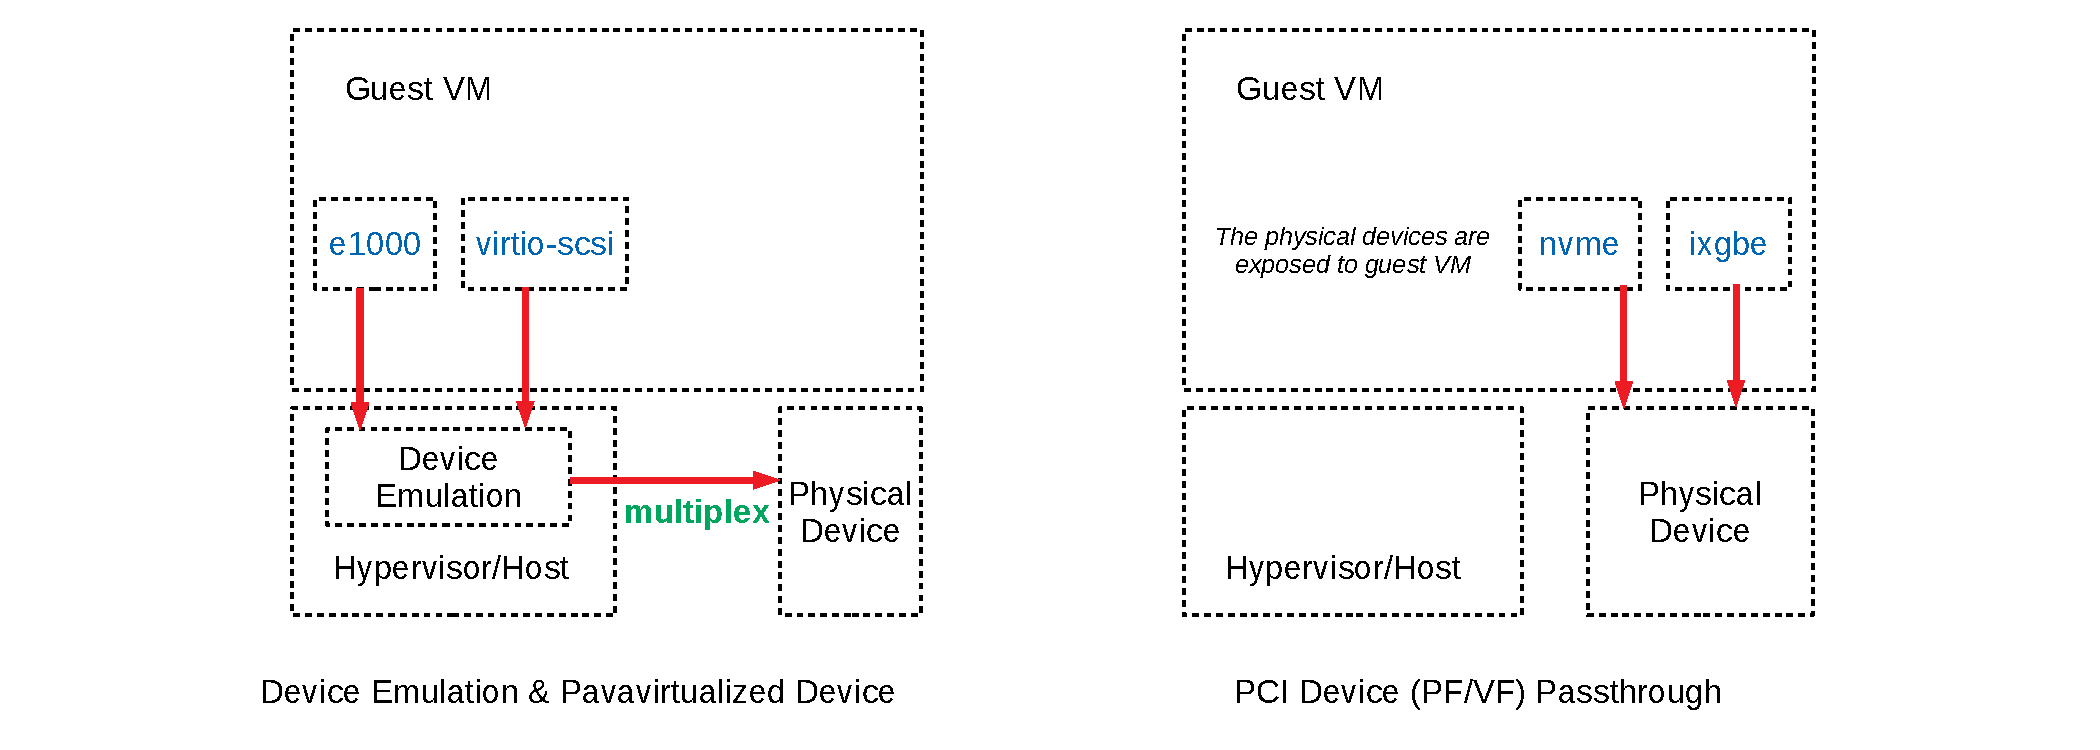
\includegraphics[width=1.0\linewidth]{figures/passthrough.pdf}
\end{figure}
\end{frame}

%------------------------------------------------

\section{KVM PCI Passthrough}
\begin{frame}
\frametitle{KVM PCI Passthrough}
\begin{block}{}
\textit{\underline{\textbf{\textcolor{red}{STEP 1}}}: To unbind \textbf{\textcolor{blue}{01:00.0}} from \textbf{NVMe} driver and register to \textbf{vfio-pci} driver:} \newline
{\small \textbf{\textcolor{blue}{01:00.0}} Non-Volatile memory controller: Intel Corporation Device f1a6 (rev 03)}

\vspace{2 mm}

host\# \textcolor{red}{echo 0000:01:00.0 $>$ /sys/bus/pci/devices/0000$\backslash$:01$\backslash$:00.0/driver/unbind} \newline
host\# \textcolor{red}{lspci -ns 0000:01:00.0} \newline
{\small 01:00.0 0108: \textbf{\textcolor{olive}{8086:f1a6}} (rev 03)}

\vspace{1 mm}

host\# \textcolor{red}{echo "\textbf{\textcolor{olive}{8086 f1a6}}" $>$ /sys/bus/pci/drivers/vfio-pci/new\_id}
\end{block}
\visible<2->{
\begin{block}{}
\textit{\underline{\textbf{\textcolor{red}{STEP 2}}}: To passthrough the VFIO-managed NVMe to QEMU/KVM VM:}

\vspace{2 mm}

{\small
\# qemu-system-x86\_64 -machine accel=kvm -vnc :0 -serial stdio -smp 4 -m 4096M \textbackslash

-net nic -net user,hostfwd=tcp::5022-:22 \textbackslash

-hda /home/user/img/boot.qcow2 \textbackslash
}

\textcolor{red}{-device vfio-pci,host=\textbf{\textcolor{blue}{0000:01:00.0}}}
\end{block}
}
\end{frame}

%------------------------------------------------

\section{Xen PCI Passthrough}
\begin{frame}
\frametitle{Xen PCI Passthrough}
\begin{block}{}
\textit{\underline{\textbf{\textcolor{red}{STEP 1}}}: To unbind \textbf{\textcolor{blue}{02:10.0}} from \textbf{igb} driver and register to \textbf{xen-pciback} driver:} \newline
{\small \textbf{\textcolor{blue}{02:10.0}} Ethernet controller: Intel Corporation I350 Gigabit Network Connection}

\vspace{2 mm}

host\# \textcolor{red}{echo 0000:02:10.0 $>$ /sys/bus/pci/devices/0000$\backslash$:02$\backslash$:10.0/driver/unbind} \newline
host\# \textcolor{red}{echo 0000:02:10.0 $>$ /sys/bus/pci/drivers/pciback/new\_slot} \newline
host\# \textcolor{red}{echo 0000:02:10.0 $>$ /sys/bus/pci/drivers/pciback/bind}


\end{block}
\vspace{4 mm}
\visible<2->{
\begin{block}{}
\textit{\underline{\textbf{\textcolor{red}{STEP 2}}}: To append below to Xen HVM config file:}

\vspace{2 mm}

\textbf{\textcolor{red}{pci = [ '02:10.0' ]}}

\end{block}
}
\end{frame}

%------------------------------------------------

\section{Virtualizatio Demo}
\begin{frame}
\frametitle{Virtualization Demo}
The virtualization demo for a new instruction set
\begin{itemize}
\item The registers (only one): \textbf{\textcolor{red}{RAX}}
\item The instructions (only one): \textbf{\textcolor{red}{mov \$7, \%rax}}
\end{itemize}
\visible<2->{\textcolor{green}{How about privileged instructions?}}
\begin{figure}
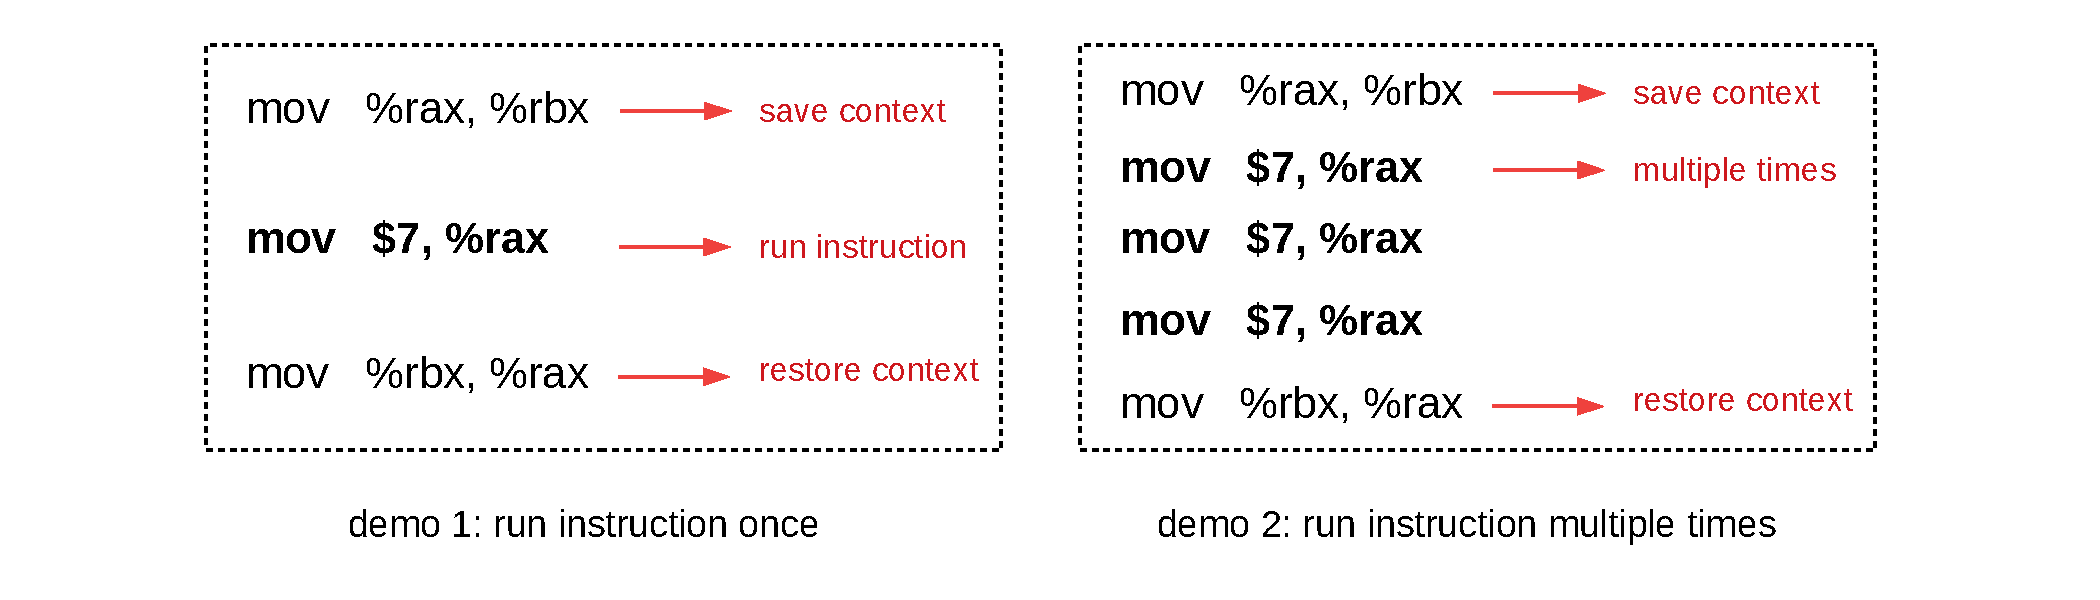
\includegraphics[width=1.0\linewidth]{figures/demo.pdf}
\end{figure}
\end{frame}

%------------------------------------------------

\section{CPU Virtualization}
\begin{frame}
\frametitle{CPU Virtualization}
\begin{itemize}
\item The CPU is divided into \textbf{\textcolor{red}{guest mode}} and regular \textbf{\textcolor{red}{host mode}}
\item Some privileged instructions are (trapped to and) emulated by \textbf{\textcolor{red}{CPU host mode}}
\item Some privileged instructions are trapped to and emulated by \textbf{\textcolor{red}{hypervisor software}}
\visible<2->{\textcolor{green}{\item How about memory virtualization?}}
\end{itemize}
\begin{figure}
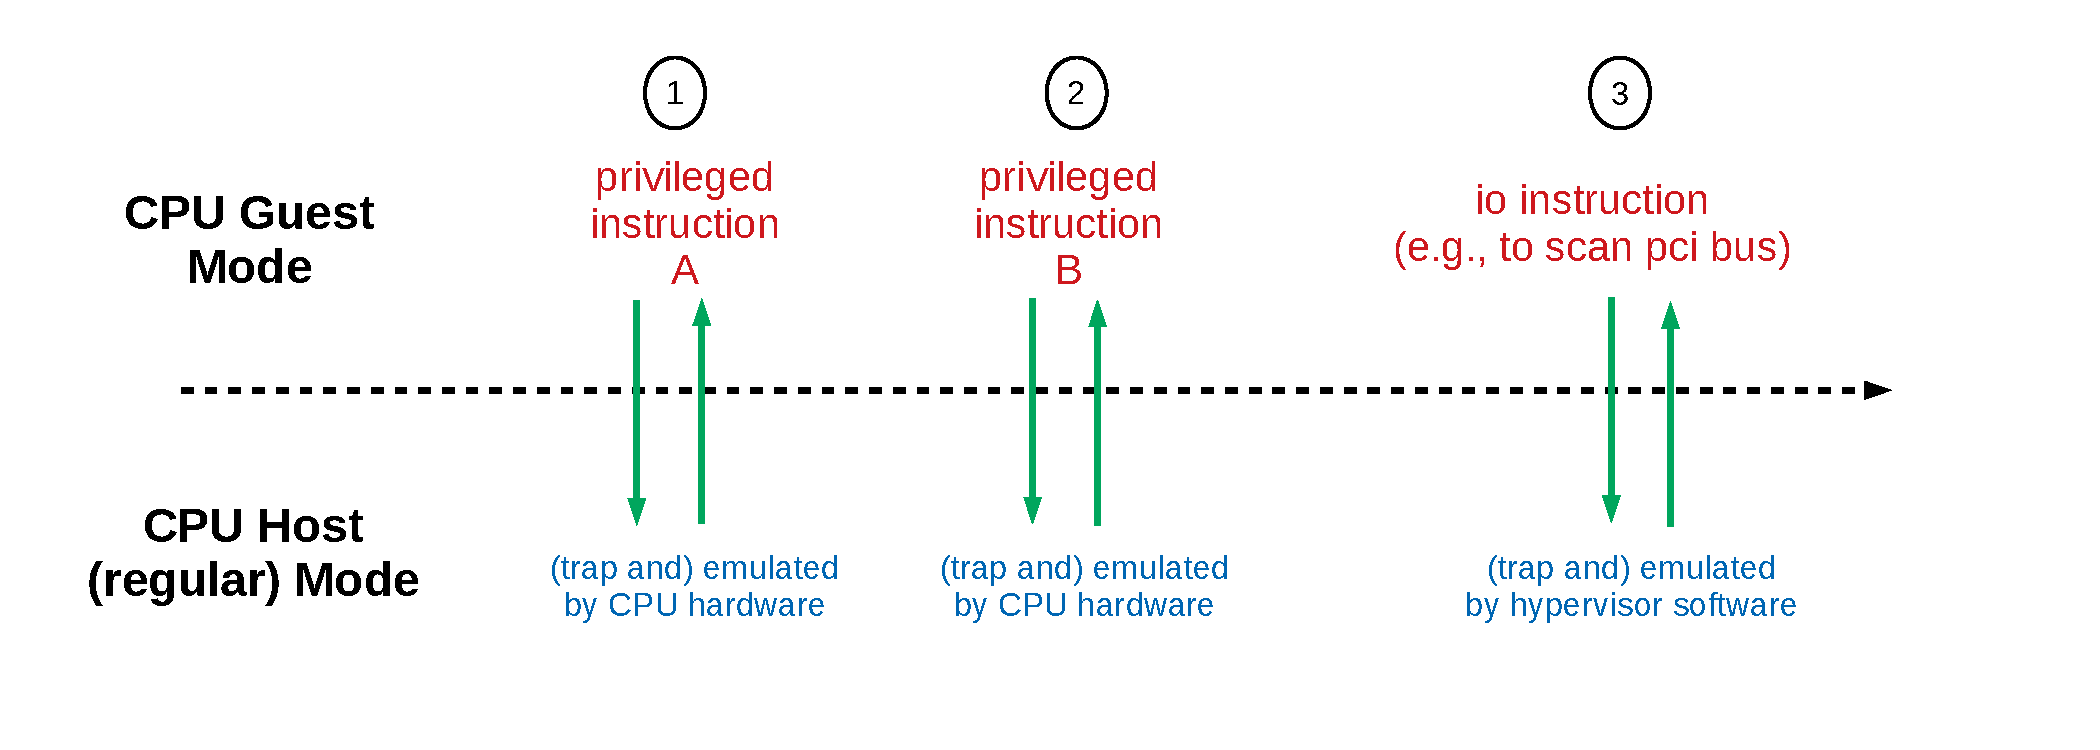
\includegraphics[width=1.0\linewidth]{figures/cpu.pdf}
\end{figure}
\end{frame}

%------------------------------------------------

\section{Memory Virtualization}
\begin{frame}
\frametitle{Memory Virtualization}
\begin{itemize}
\item \textbf{\textcolor{red}{Guest Page Table (CR3)}}: Guest Virtual Address to Guest Physical Address
\item \textbf{\textcolor{red}{Host Page Table (EPTP)}}: Guest Physical Address to Host Physical Address 
\item To set EPT entry as non-read, non-write or non-exec can trap guest VM memory access
\end{itemize}
\begin{figure}
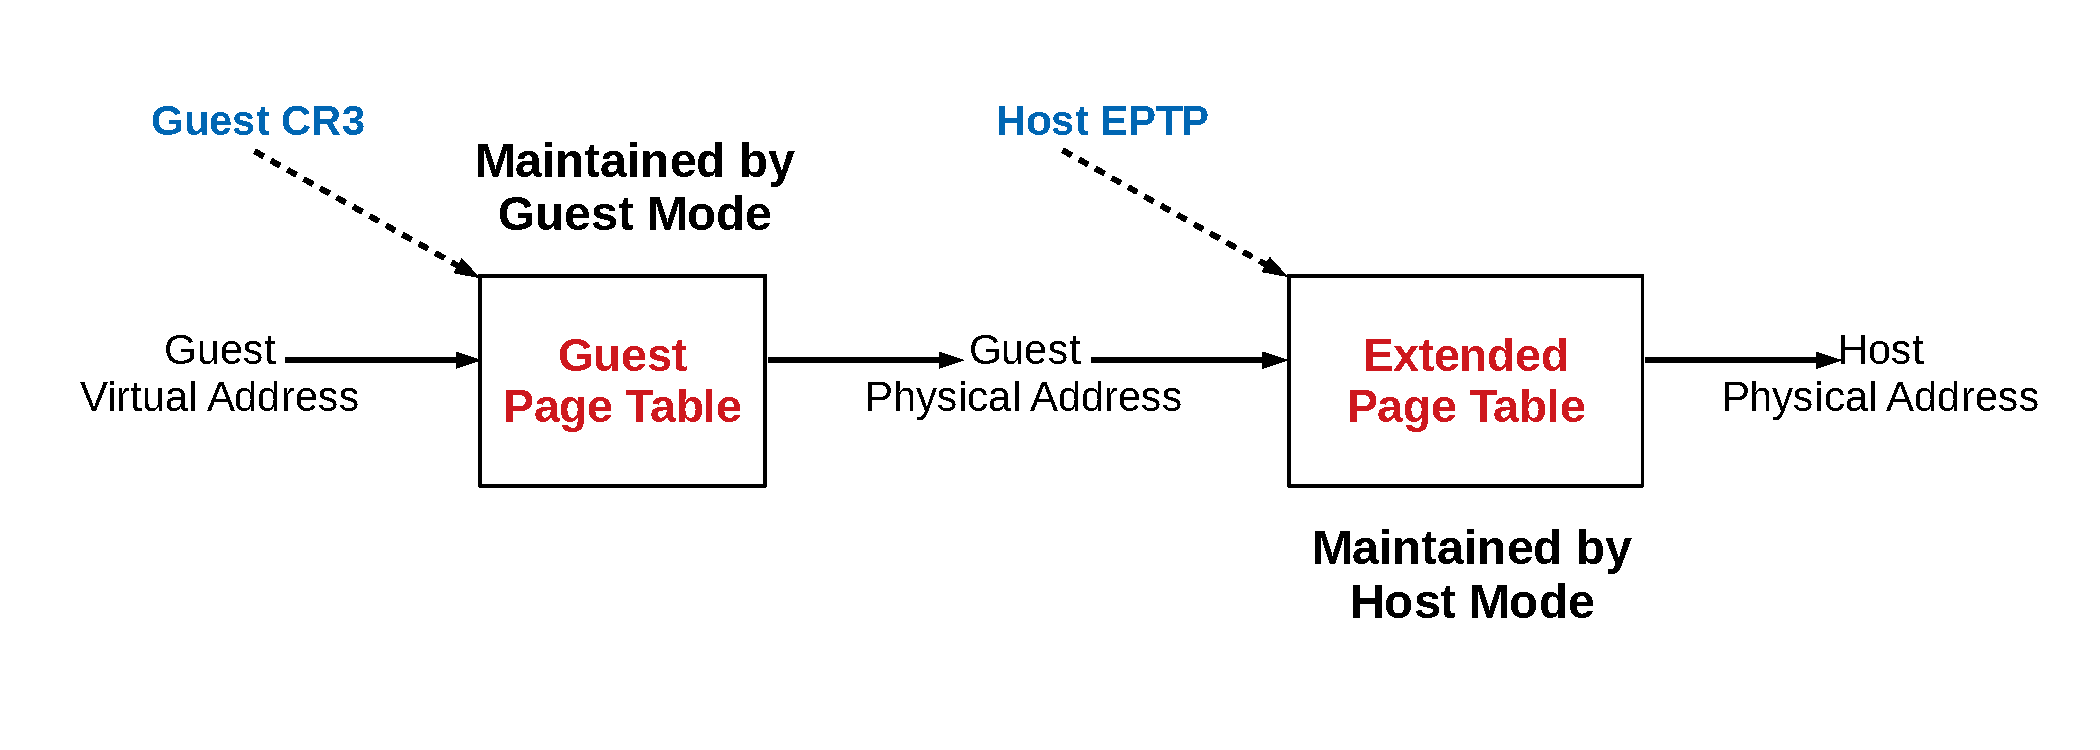
\includegraphics[width=1.0\linewidth]{figures/memory.pdf}
\end{figure}
\end{frame}

%------------------------------------------------

\section{PCI Device Emulation 1/2}
\begin{frame}
\frametitle{PCI Device Emulation 1/2}
\begin{itemize}
\item PCI: \textbf{\textcolor{red}{config space}}, \textbf{\textcolor{red}{capabilities}} and \textbf{\textcolor{red}{bar}}
\item The PCI Bar is usually to register DMA ring buffer, configure MSI-X and kick doorbell
\end{itemize}
\begin{figure}
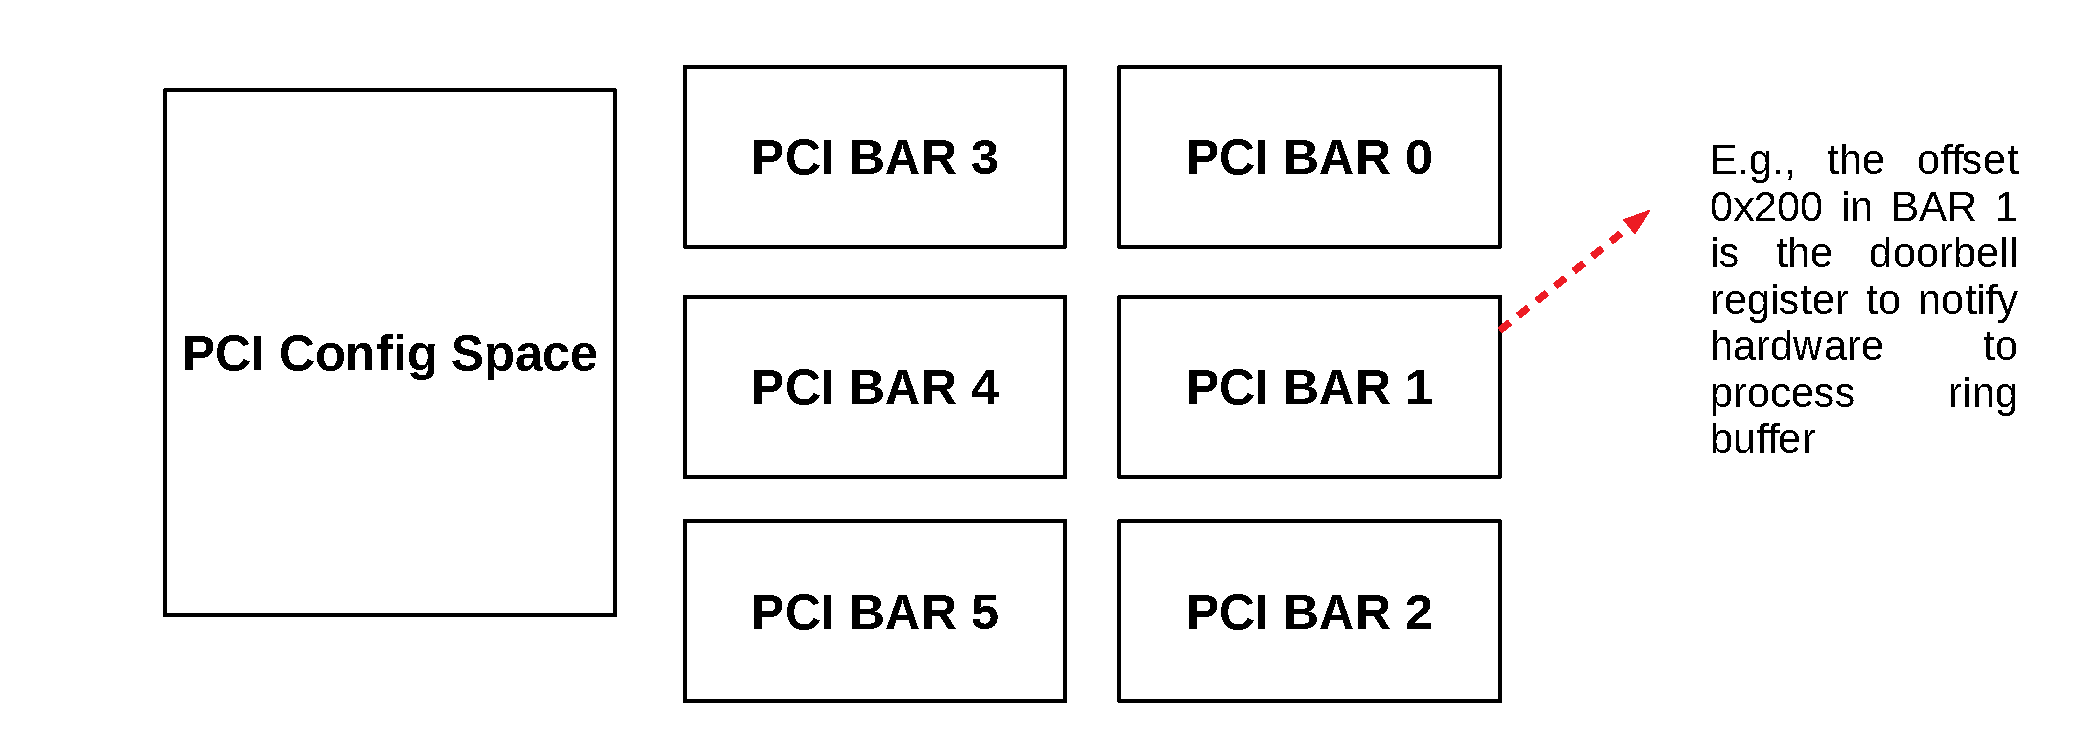
\includegraphics[width=1.0\linewidth]{figures/pci_spec.pdf}
\end{figure}
\end{frame}

%------------------------------------------------

\section{PCI Device Emulation 2/2}
\begin{frame}
\frametitle{PCI Device Emulation 2/2}
\begin{itemize}
\item EPT is configured on purpose to trap \textbf{\textcolor{red}{MMIO}} bar access
\item PCI (config/bar) access by \textbf{\textcolor{red}{IO}} instruction is trapped to hypervisor
\item Both \textbf{IO} and \textbf{MMIO} are emulated by hypervisor
\end{itemize}
\begin{figure}
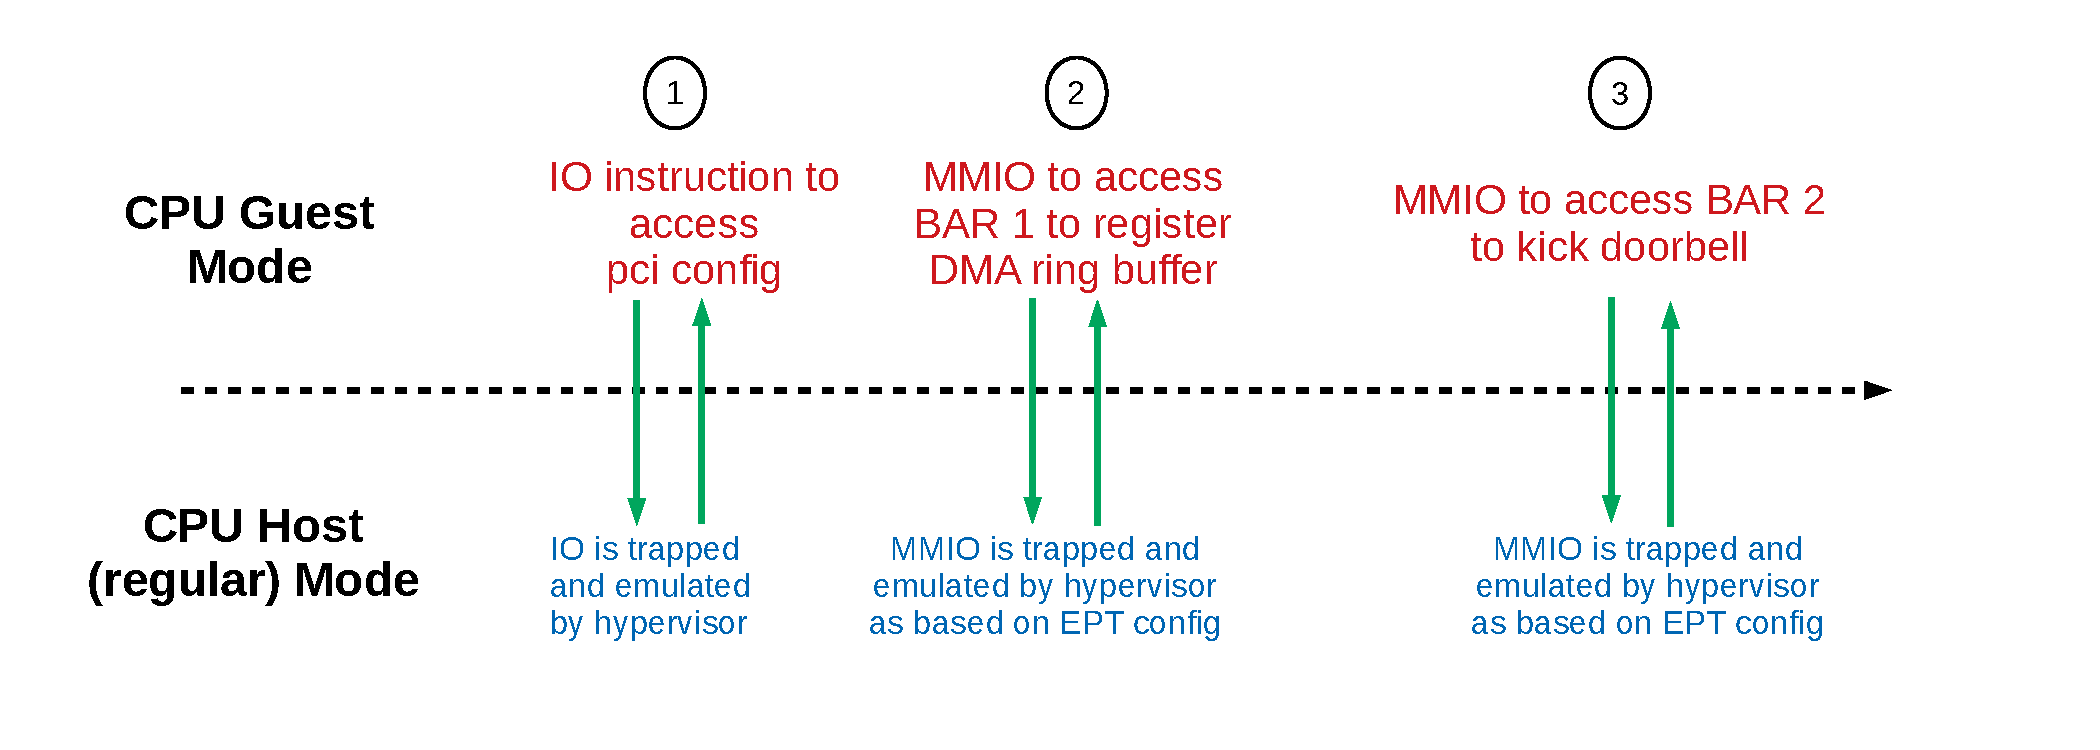
\includegraphics[width=1.0\linewidth]{figures/pci_access.pdf}
\end{figure}
\end{frame}

%------------------------------------------------

\section{PCI Passthrough 1/4: Plan A}
\begin{frame}
\frametitle{PCI Passthrough 1/4: Plan A}
\begin{itemize}
\item Hypervisor as intermediate layer:
\begin{itemize}
\item Access to PCI config/bar is always trapped to hypervisor
\item Hypervisor access PCI device and propagate result to VM
\end{itemize}
\visible<2->{\item Cons: too many traps to hypervisor!}
\end{itemize}
\begin{figure}
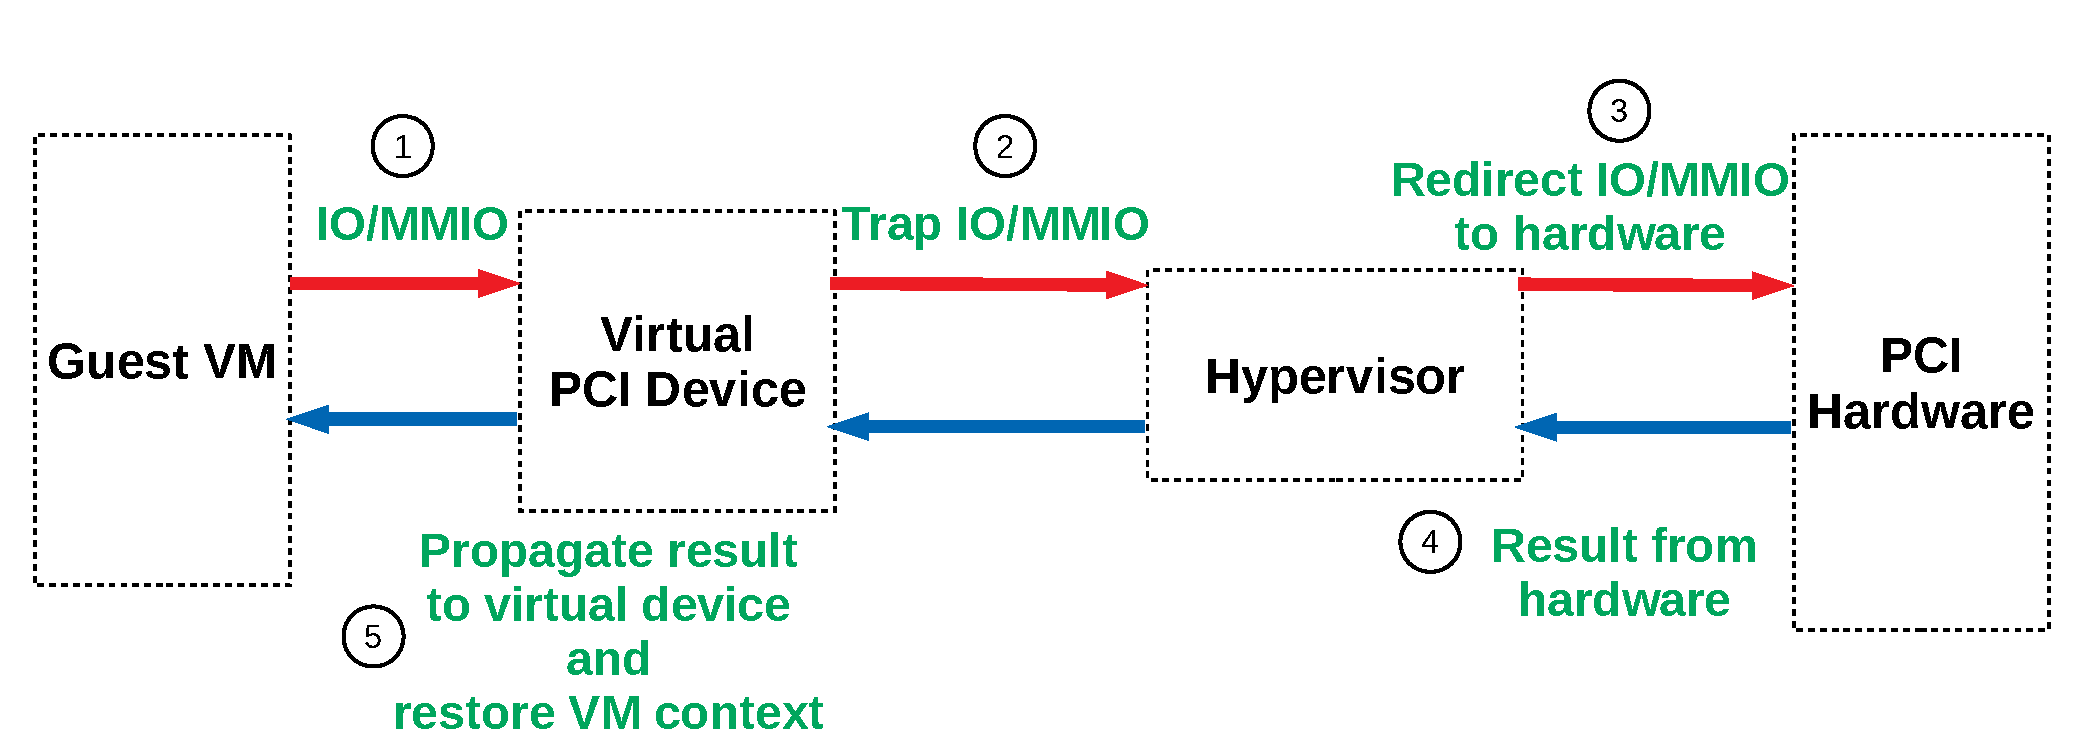
\includegraphics[width=1.0\linewidth]{figures/plan_a.pdf}
\end{figure}
\end{frame}

%------------------------------------------------

\section{PCI Passthrough 2/4: Plan B}
\begin{frame}
\begin{itemize}
\item The hypervisor maps PCI config/bars into VM address space via EPT
\item The VM has direct mmio access to PCI config/bars to avoid \textbf{trap}
\visible<2->{\item Q1: DMA is based on HPA, NOT GPA!}
\visible<3->{\item Q2: MSI-X IRQ is based on host CPU ID, NOT guest CPU ID!}
\end{itemize}
\frametitle{PCI Passthrough 2/4: Plan B}
\begin{figure}
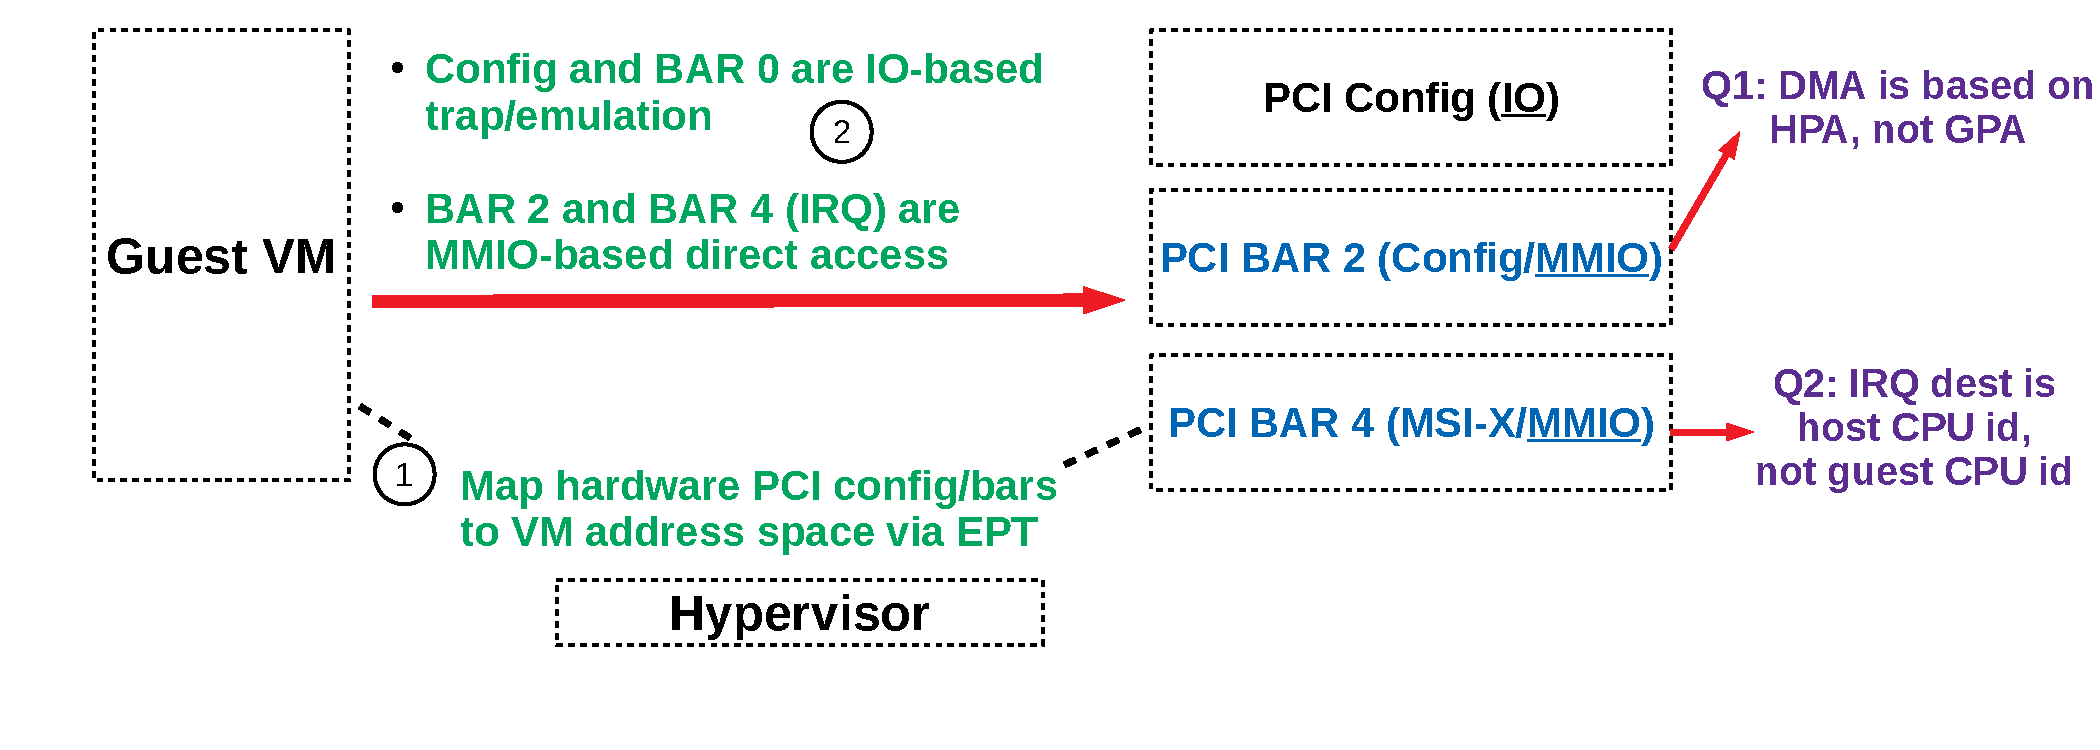
\includegraphics[width=1.0\linewidth]{figures/plan_b.pdf}
\end{figure}
\end{frame}

%------------------------------------------------

\section{PCI Passthrough 3/4: Plan C}
\begin{frame}
\frametitle{PCI Passthrough 3/4: Plan C}
\begin{itemize}
\item Map some PCI BARs (e.g., ring buffer base or doorbell) to VM address space
\item Access to PCI config and MSI-X table is trapped to hypervisor
\item Redirect IRQ from PCI device to VM via hypervisor
\visible<2->{\item Q1: DMA is based on HPA, NOT GPA! (Device Isolation across VMs)}
\end{itemize}
\begin{figure}
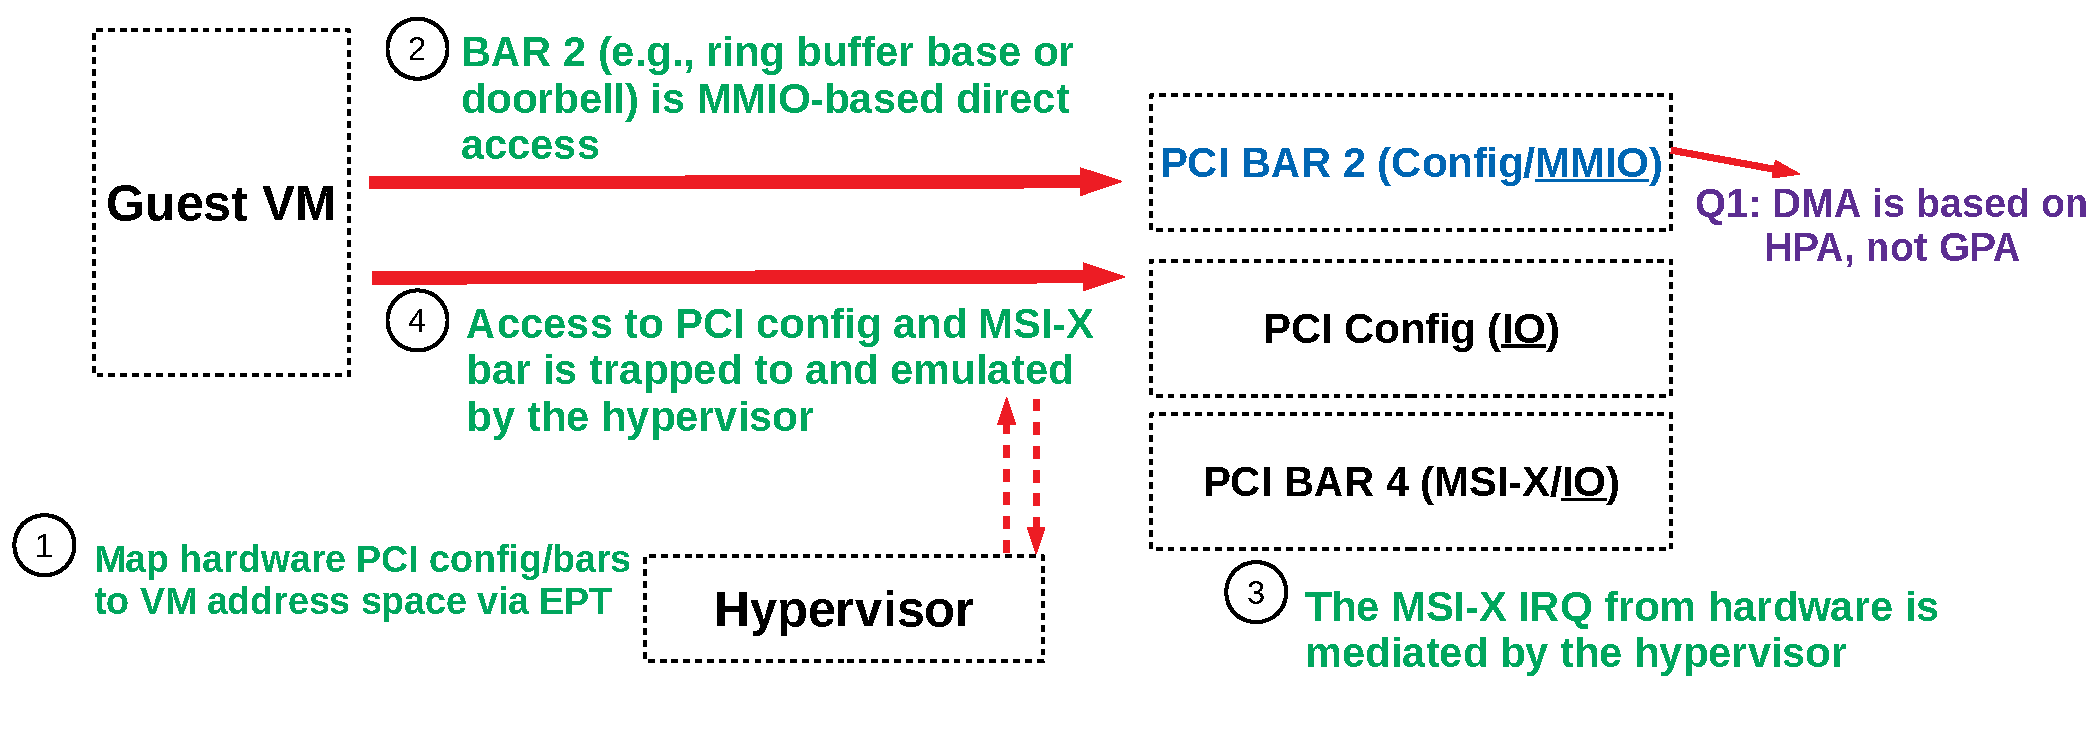
\includegraphics[width=1.0\linewidth]{figures/plan_c.pdf}
\end{figure}
\end{frame}

%------------------------------------------------

\section{PCI Passthrough 4/4: Plan D}
\begin{frame}
\frametitle{PCI Passthrough 4/4: Plan D}
\begin{itemize}
\item Map some PCI BARs (e.g., ring buffer base or doorbell) to VM address space
\visible<2->{\item Access to PCI config and MSI-X table is trapped to hypervisor}
\visible<3->{\item Redirect DMA GPA to HPA via IOMMU}
\visible<4->{\item Redirect IRQ from PCI device to VM via hypervisor/IOMMU}
\end{itemize}
\begin{figure}
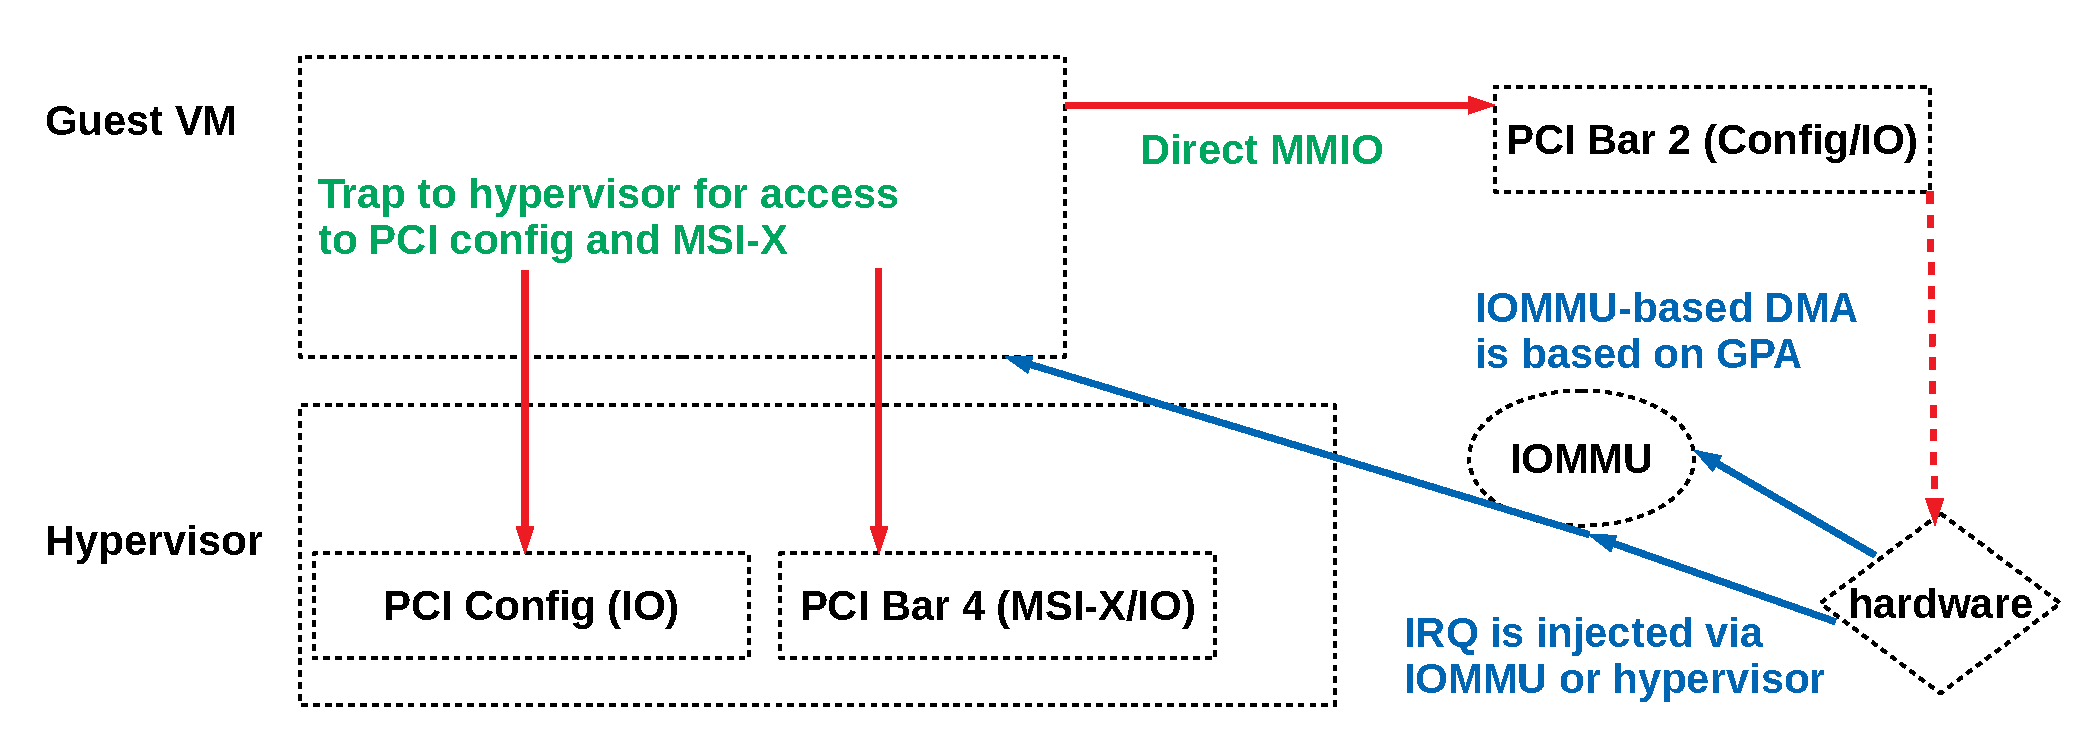
\includegraphics[width=1.0\linewidth]{figures/plan_d.pdf}
\end{figure}
\end{frame}

%------------------------------------------------

\section{KVM PCI Passthrough Memory Mapping 1/2}
\begin{frame}
\frametitle{KVM PCI Passthrough Memory Mapping 1/2}
\begin{figure}
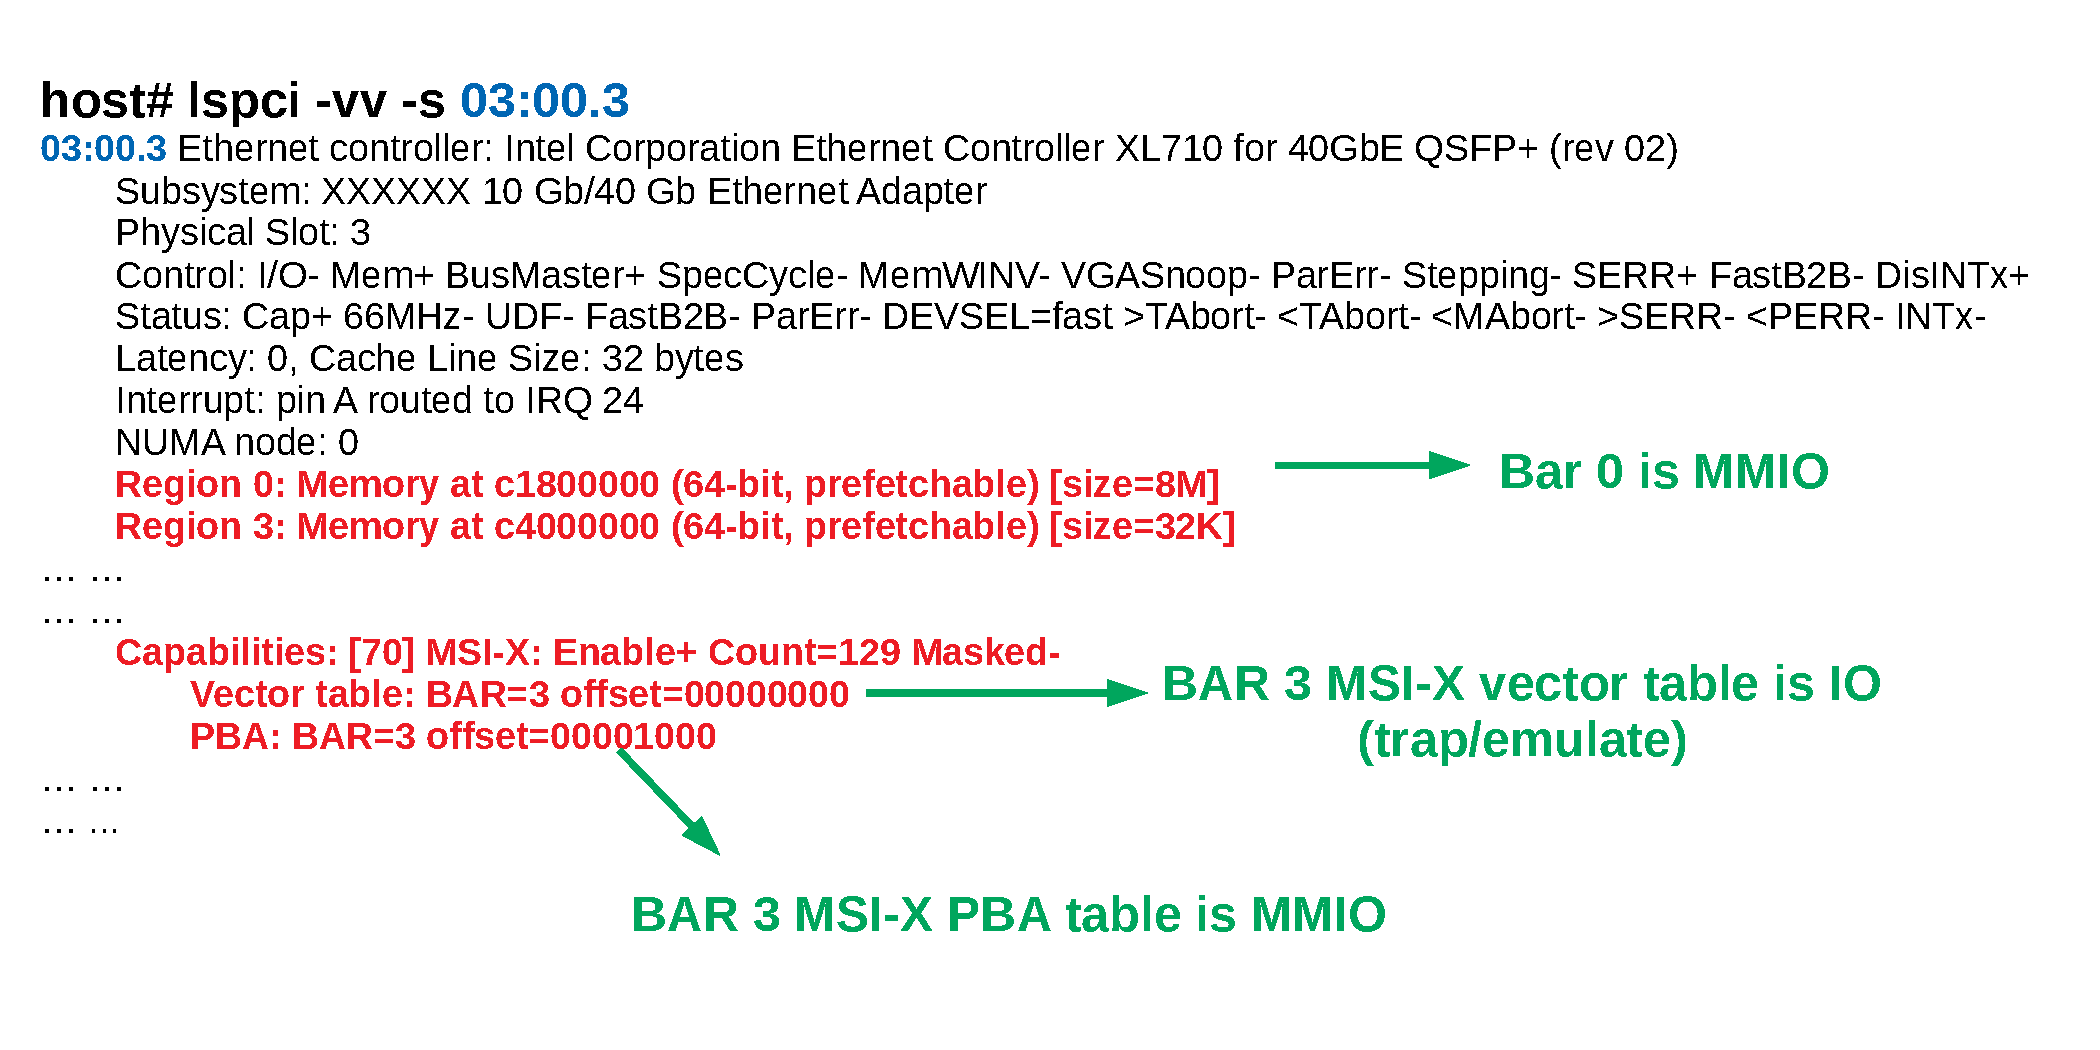
\includegraphics[width=1.0\linewidth]{figures/lspci.pdf}
\end{figure}
\end{frame}

%------------------------------------------------

\section{KVM PCI Passthrough Memory Mapping 2/2}
\begin{frame}
\frametitle{KVM PCI Passthrough Memory Mapping 2/2}
\begin{figure}
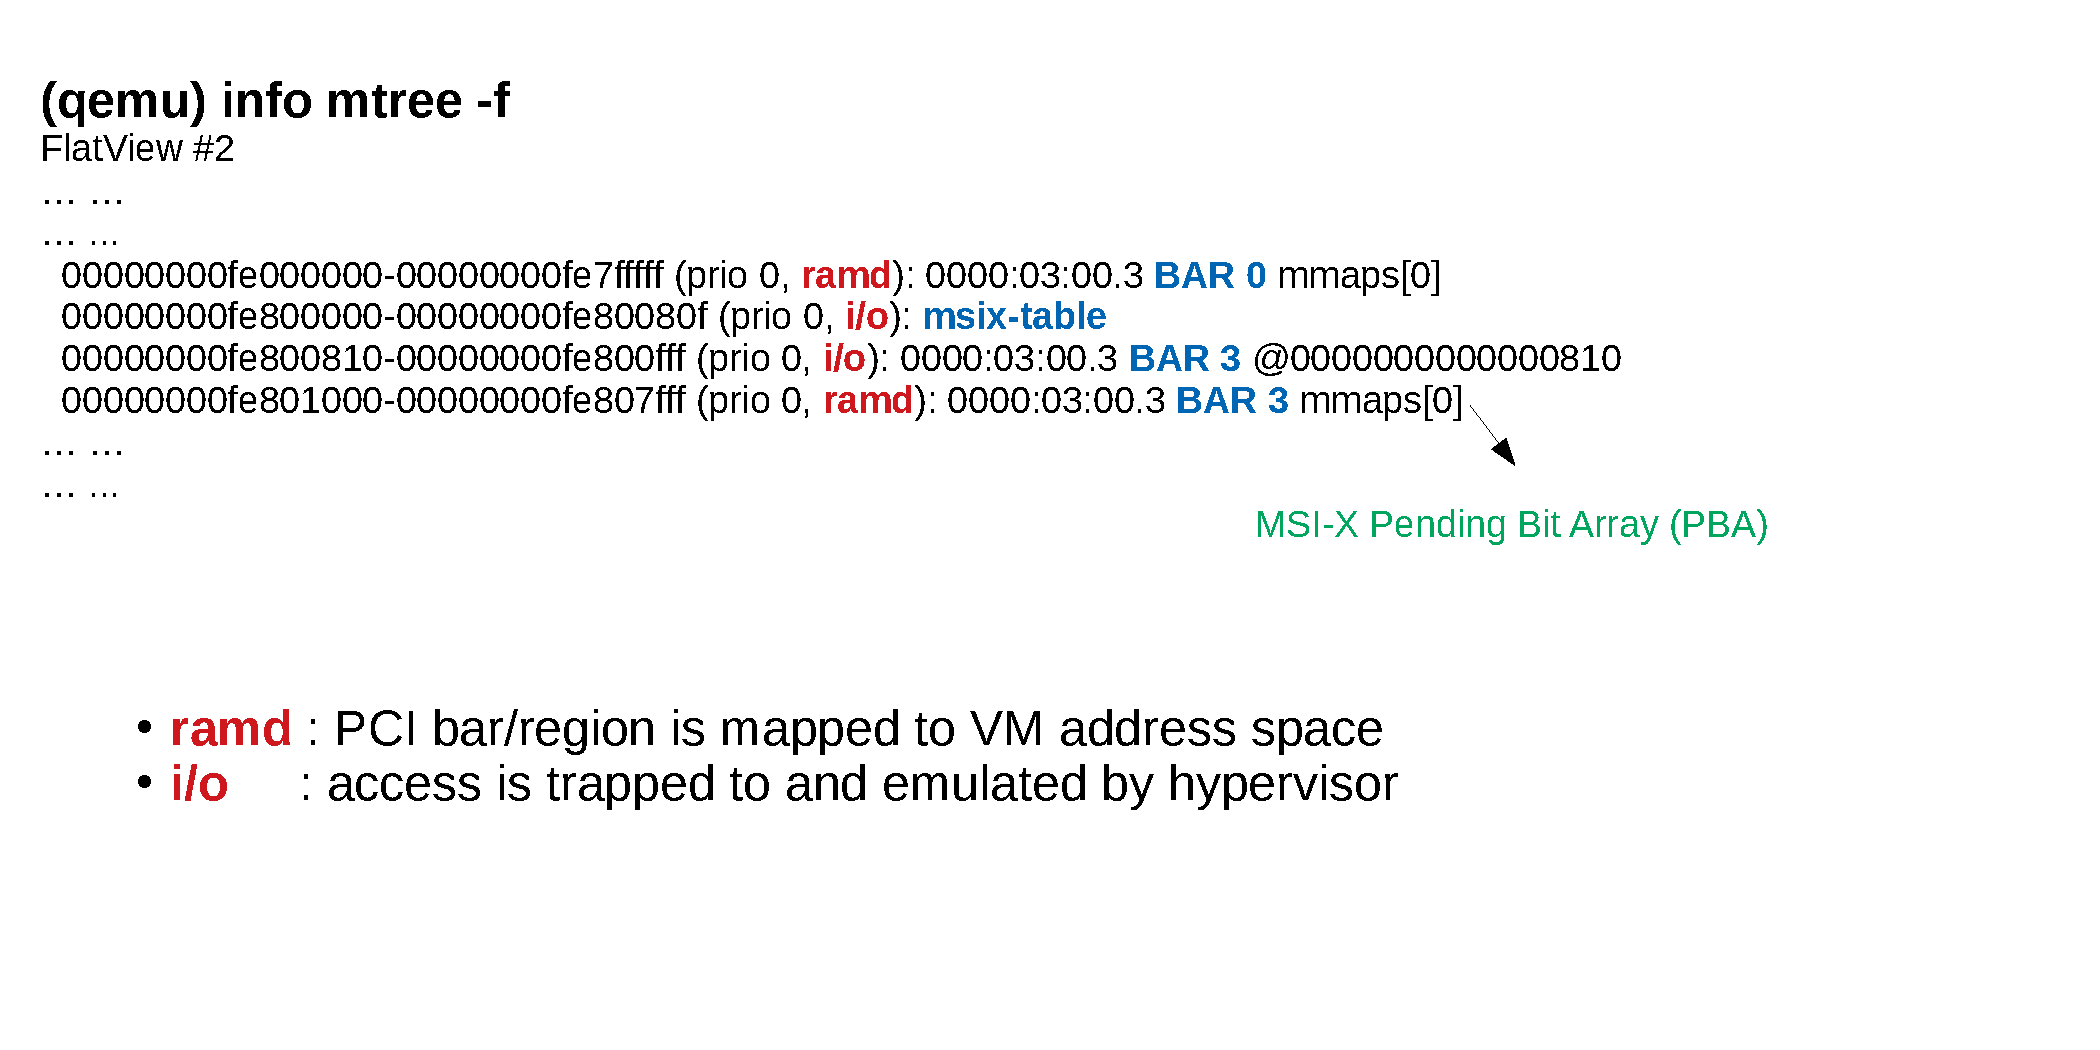
\includegraphics[width=1.0\linewidth]{figures/flatview.pdf}
\end{figure}
\end{frame}

%------------------------------------------------

\section{Bridge the Gap}
\begin{frame}
\frametitle{Bridge the Gap}
\begin{figure}
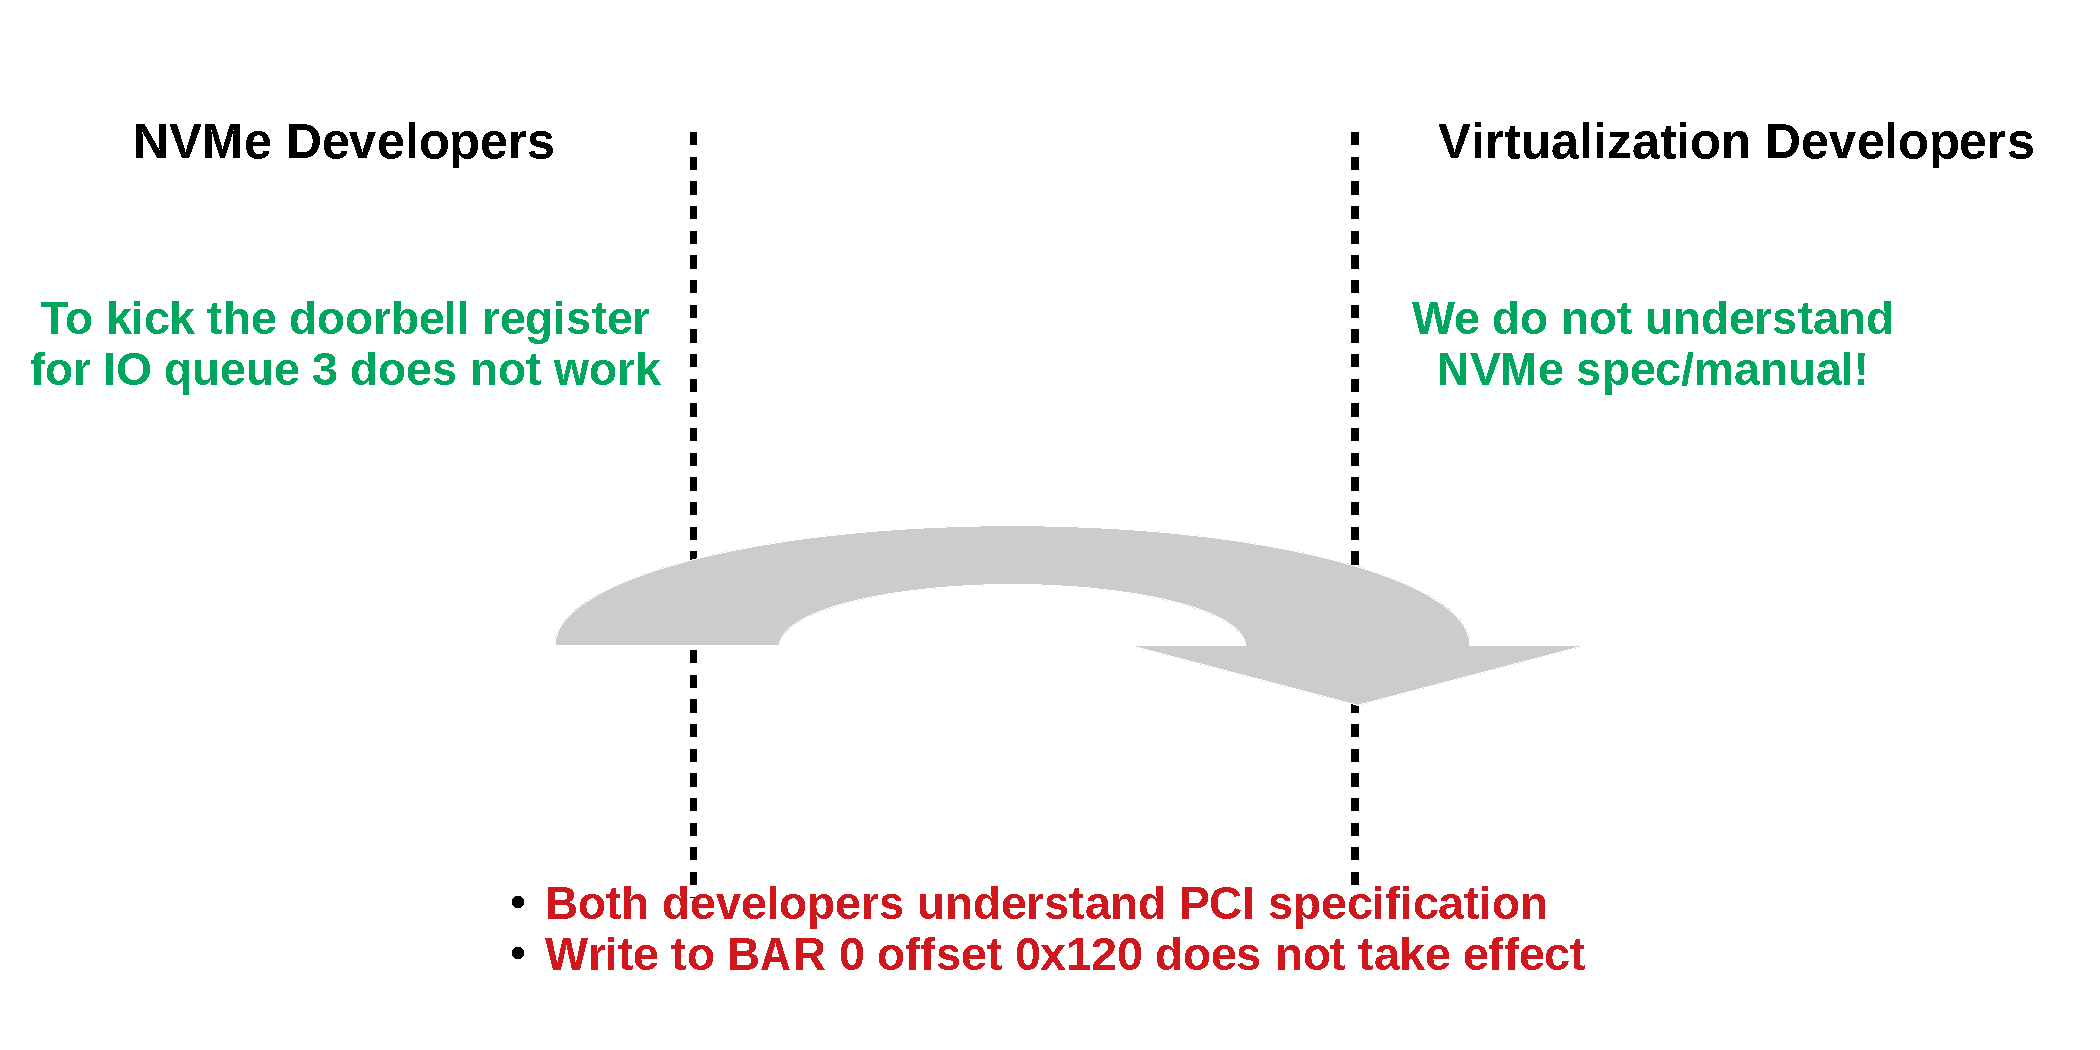
\includegraphics[width=1.0\linewidth]{figures/bridge.pdf}
\end{figure}
\end{frame}

%------------------------------------------------

\section{Take-Home Message}
\begin{frame}
\frametitle{Take-Home Message}
\begin{itemize}
\item Virtualization is \textbf{trap and emulation} (explicitly by software or implicitly by hardware)
\visible<2->{\item PCI Passthrough is \textbf{to reduce the cost a PCI device is accessed by VM}, via:}
\begin{itemize}
\visible<2->{\item Map some PCI BARs (e.g., ring buffer base or doorbell) to VM address space}
\visible<3->{\item Access to PCI config and MSI-X table is trapped to and emulated by hypervisor}
\visible<4->{\item Redirect DMA GPA to HPA via IOMMU}
\visible<5->{\item Redirect IRQ from PCI device to VM via hypervisor/IOMMU}
\end{itemize}
\visible<6->{\item To bridge the gap (between NVMe/Ethernet/IB and virtualization) via PCI spec}
\visible<7->{\item Congratulations! You have learned about to implement virtualization demo from scratch!}
\end{itemize}
\end{frame}

%------------------------------------------------

%\begin{frame}
%\Huge{\centerline{The End}}
%\end{frame}

%----------------------------------------------------------------------------------------

\end{document} 
